%WRITTEN BY: Daniel
\subsection{Deployment}

\subsubsection{Architecture}\hfill\\
Every configuration management tool requires an architecture which supports the management of a set of hosts. A popular architecture is illustrated in Figure \ref{fig:architecture} where a centralized control server manages the configuration and an agent program is installed on every managed device. The centralized control server is responsible to keep a canonical state of configuration as provided by the operator in a repository and translates the configuration into profiles for every node.

\begin{figure*}
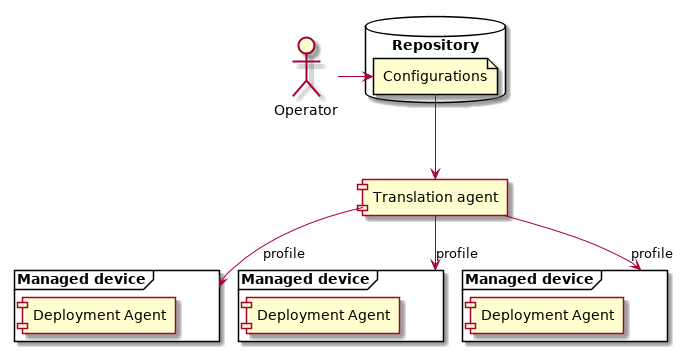
\includegraphics[height=2in]{assets/architecture}
\caption{Architecture of a centralized configuration management tool \cite{delaet2010survey}}
\label{fig:architecture}
\end{figure*}

\begin{table}[H]
\begin{tabular}{lll}
\toprule
Component & Chef & Puppet \\
\midrule
Translation Agent  & Chef Server  & Puppet Master \\
Deployment Agent & Chef Client & Puppet Agent \\
\end{tabular}
\label{tbl:components}
\end{table}

Chef and Puppet both follow this pattern and the only differ in terms of technology for implementing the architecture and the terminology used (See Table).

\subsubsection{Distribution Mechanism}\hfill\\
In order to distribute configurations from the centralized control server there are two mechanisms tools implement.

\begin{description}
	
	\item[Push-based systems] \hfill \\ 
	Configuration is pushed and synchronously applied on the managed hosts. This does not require an agent program to be installed on the machine. 
	
	\item[Pull-based systems] \hfill \\
	Configuration is fetched by the agent program from the centralized control server in regular intervals and changes are applied by the agent program.
	
\end{description}


Chef and Puppet both are pull-based systems because it has been shown that the pull-based approach scales better to a large number of managed hosts but both CM tools have implemented capabilities to manually trigger configuration distribution outside of the regular pull-schedule. For Chef the \textit{Push Jobs} extension allows jobs to be run independently from the periodic configuration convergence. Puppet allows for similiar behaviour through external orchestration tools such as MCollective \cite{mcollective}.

\subsubsection{Platform Support}\hfill\\

Both Chef and Puppet support a number of different platforms for running their agent programs such as AIX, FreeBSD, Solaris, Linux, macOS and Windows. The control server needs to be run on a Linux-based system for both tools.
